\section{Email Forwarding in Practice}
% \section{The Challenges with Email Forwarding}
\label{sec:measure_forwarding_mechs_and_arc}

Despite the ubiquity of email forwarding, there is no single and
universally agreed-upon method for how email services should implement
forwarding, resulting in several different approaches~\cite{Emailfor34:online}.  This
heterogeneity stems in part from the difficulty of balancing
compatibility with anti-spoofing protocols and the functional goals of
many forwarding use cases: to transparently hide the intermediate
forwarder and present the illusion that the recipient receives the
email directly from its original sender.

Absent a clear standard to depend on, we have used empirical
measurements to \emph{infer} the forwarding behavior deployed by
prominent email providers and mailing list services.  For each
service, we created multiple test accounts, used them to forward email
to recipient accounts we controlled, and then analyzed the resulting
email headers to identify the forwarding mechanism employed.
(Section~\ref{sec:methodology} has a more detailed description of our
methodology.)

We constructed a comprehensive and representative set of forwarding services by building on top of prior literature.
In total, we studied 20 distinct, leading email forwarding services.
We started by collecting all email providers studied in prior literature~\cite{chen2020composition,shen2020weak,hu_end--end_nodate,wang2022revisiting}.
We considered an email provider \emph{out of scope} if it meets any of these four criteria: (a) it is no longer active (e.g., excite.com); (b) it does not accept US customers (e.g., all Chinese providers studied in prior work);  (c) it is not open to public registration (e.g., cock.li); or (d) it does not support forwarding (e.g., Protonmail).
Using these criteria, we identified 23 email providers.
Next, we excluded five email providers that prohibited bulk registration (which prevents us from running large-scale measurements), leaving us with 18 email providers.
We then identified and removed duplicate providers that are operated by the same vendor under different names, leading to a total of 14 distinct email providers.
Finally, we augmented this set of forwarding services by searching for popular email providers that supported forwarding and widely-used mailing list services (a common use case overlooked in prior literature), adding two additional email providers (Mail2World and GoDaddy) and four mailing lists.

Our selection of email forwarding services covers a diverse set of countries and real-world use cases (personal and business email), and represents services used by the general public (used by over 46\% of popular Alexa domains and government domains according to Liu et al.~\cite{liu2021s} ignoring email filtering services).
%\alex{42.7\% considering email filtering}. 
We list all email providers and mailing lists in Table~\ref{tab:forwarding_mechs_in_the_wild}.


Through our measurements, we confirmed the use of three common
approaches that are generally known through public documentation, and
identified a fourth uncommon implementation used by
Microsoft Outlook (hence referred to as Outlook) and Freemail.hu (hence referred to as Freemail).
As summarized in
Figure~\ref{fig:forwarding_mechs_combined}, in each approach the
forwarder modifies the sender and recipient fields in the SMTP
Envelope and Message headers before relaying the email to its
recipient.



% By analyzing public documentation and empirically testing popular email services (\S~\ref{sec:fwd_adoption_measurement}), we identified four major approaches to implementing email forwarding.
% \geoff{is this a ``result'' because Microsoft's implementation has to be experimentally discovered?}\alex{it is technically discovered through experiments}

We now describe each of these approaches in detail using two running
examples of common email forwarding use cases.  In the first case,
Alice has configured her university account (\dns{alice@univ.edu}) to
forward to her primary personal account (\dns{alice@gmail.com}).  When
her university account receives email (\eg, from
\dns{sp@hotcrp.com}), forwarding retransmits it to
\dns{alice@gmail.com} in a way that makes it seem like the email comes
directly from the sender (\dns{sp@hotcrp.com}), rather than from her
university account.  In the second case, Bob sends an email to a
mailing list (\dns{list@univ.edu}), which redistributes (forwards) the
email to the list's members (\eg, \dns{user@univ.edu}).


\begin{figure}[t]
  \centering
%  \vspace*{-0.1in}
    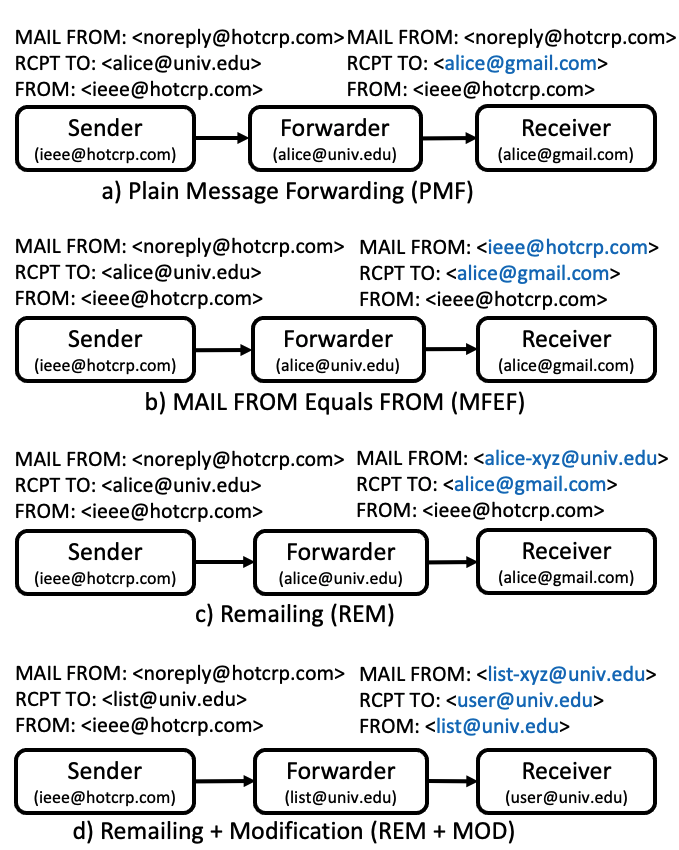
\includegraphics[width=0.7\columnwidth]{fig/table_forwarding_mechanisms_combined.pdf}
    \caption{Four prevalent approaches to email forwarding.  Addresses
      in blue correspond to header values rewritten during the
      forwarding process.
      }
    \label{fig:forwarding_mechs_combined}
\end{figure}


% \grant{In MFEF, is there a reason why the MAILFROM is acm instead of hotcrp? If it's to illustrate a change, I suggest we use noreply@hotcrp.com for the sender MAIL FROM addresses.}\alex{fixed}

% \noindent{\bf Plain Message-Forwarding (PMF)}.
\textbf{Plain Message-Forwarding (PMF)}. Initially designed for
the purpose of ``source-routing''~\cite{Emailfor45:online}, PMF was
one of the first forwarding mechanisms in wide use.
Forwarders that use PMF only change
the \textsc{RCPT TO} header from the forwarder's email account (\dns{alice@univ.edu}) to the final recipient's address (\dns{alice@gmail.com}), and leave all other fields
untouched,
%~\cite{Emailfor45:online},
as illustrated in Figure~\ref{fig:forwarding_mechs_combined}a.
This approach achieves the goal of transparent forwarding.
Changing the \textsc{RCPT TO} header will tell mail servers to send the email to the new address's account, and leaving the \textsc{FROM} header intact will
cause the recipient's email client to display the initial sender (\dns{sp@hotcrp.com}),
rather than presenting \dns{alice@univ.edu} as the sender.
% This approach achieves the goal of transparent forwarding, since the email will appear to come from its initial sender (the \textsc{FROM} header displays the original sender).
% However, it will cause SPF validation to fail in many cases, since the \textsc{MAIL FROM} domain may not list the forwarding server's IP address in its SPF allowlist.


% \noindent{\bf MAIL FROM Equals From (MFEF)}.
\textbf{MAIL FROM Equals FROM (MFEF)}.
Similar to PMF, MFEF (Figure~\ref{fig:forwarding_mechs_combined}b) aims to achieve transparent forwarding by preserving the original sender's identity in the \textsc{FROM} header.
Unlike the other forwarding approaches described in this section, MFEF is a custom forwarding implementation that appears to be used only by Outlook and Freemail.
% \footnote{We are not
%   entirely clear what function MFEF serves but we hope, as part of our
%   disclosure interactions with Microsoft, to gain a better
%   understanding of this design's motivation for a future version of
%   this paper.}
A MFEF forwarder not only rewrites the \textsc{RCPT TO} header to the final recipient (\dns{alice@gmail.com}), but it \emph{also} sets the \textsc{MAIL FROM}
header to be the same as the \textsc{FROM} header (from \dns{noreply@hotcrp.com} to \dns{sp@hotcrp.com}).

Email forwarded using PMF and MFEF often break SPF validation because the \textsc{MAIL FROM} domain typically does not list the forwarding server's IP address in its SPF allowlist;
in our example, \dns{hotcrp.com} does not list the email servers for \dns{univ.edu} in its SPF allowlist.
This incompatibility has hindered the adoption of SPF and DMARC~\cite{hutowardsunderstanding},
leading to provider-specific defenses and new anti-spoofing protocols that we describe in Section~\ref{sec:assumptions}.

%Despite these defenses, we show how attackers can abuse forwarding to nonetheless successfully spoof email from hundreds of thousands of popular domains in
%Section~\ref{sec:attacks}.

% Figure~\ref{fig:forwarding_mechs_combined}a depicts the actions of
% such a forwarder which changes the \textsc{RCPT TO} header to the
% address of the receiver (\dns{c@c.com}) and leaves all other fields
% intact.

% In general, SPF disallows PMF, since this style of forwarding often
% causes SPF checks to fail at the final receiver.  Nevertheless, as we
% detail later, many email providers, like Yahoo and Fastmail, still use
% PMF in practice, which can result in security issues.

% {\bf Remailing (REM)}.
\textbf{Remailing (REM)}. Unlike PMF and MFEF, remailing (aka redistribution)
works well with SPF because this approach alters the headers in a way that resembles the action of the forwarder submitting a new message~\cite{SenderRe69:online}.
% It refers to re-sending a message and also
% rewriting the \textsc{MAIL FROM} field. It is commonly named remailing
% because the process resembles the action of a Mail User Agent
% submitting a new
% message\cite{SenderRe69:online}.
As shown in Figure~\ref{fig:forwarding_mechs_combined}c, the REM
forwarder (\dns{univ.edu}'s mail server) first changes the
\textsc{RCPT TO} header to specify the final recipient (\dns{alice@gmail.com}).
Additionally, the forwarder rewrites the \textsc{MAIL FROM} header so that it
corresponds to an address in the forwarder's own domain (\eg,
\dns{alice-xyz@univ.edu}).\footnote{The Sender Rewriting Scheme
(RFC~5231~\cite{rfc5231})provides a generic framework for how forwarders should
rewrite the \textsc{MAIL FROM} header.  However, email providers do not
strictly follow this scheme and the exact email address after rewriting varies
by implementation.}
% \footnote{The exact username of the \textsc{MAIL FROM} address after
% rewriting varies by the specific implementation.}  The Sender Rewriting
% Scheme, defined in RFC 5231~\cite{rfc5231}, provides a generic
% framework for rewriting email addresses in the \textsc{MAIL FROM}
% header. However, in reality, providers do not strictly follow this
% scheme.

However, even though REM interoperates with SPF, it can still fail DMARC
authentication.  Absent a valid DKIM header, email messages forwarded
via REM will fail DMARC's alignment test because the \textsc{FROM}
domain will not match the SPF-verified \textsc{MAIL FROM}
domain.\footnote{Many domains still do not implement DKIM for outbound email, and even
  those that do can have their user's DKIM signatures invalidated by mailing
  list software that adds content to a user's post~\cite{rfc6783}.}
This incompatibility has led to the common adoption of weaker DMARC policies,
such as \textsc{None} and \textsc{Quarantine} instead of
\textsc{Reject}~\cite{hutowardsunderstanding}.

% This creates a problem if the \textsc{FROM}
% domain has strict DMARC policies like quarantine or reject.

% \noindent{\bf Remailing with Modification (REM + MOD)}.
\textbf{Remailing with Modification (REM + MOD)}.
The final forwarding approach, Remailing with Modification (REM + MOD)~\cite{rfc6783},
resolves these compatibility issues by sacrificing the goal of transparent forwarding.
Email forwarded using REM + MOD will pass both SPF and DMARC.
However, email forwarded with this approach will display the \textit{forwarder} as the email's sender to the final recipient (hiding the identity of the original sender).
Because of this functional change, most major email platforms do not adopt this approach, and it is used primarily by mailing list services such as Gaggle.

As shown in Figure~\ref{fig:forwarding_mechs_combined}d, with REM + MOD the forwarder modifies the headers just like it would during REM forwarding: changing the \textsc{RCPT TO} header to the final recipient (\dns{user@univ.edu}) and the \textsc{MAIL FROM} header to an address in the forwarder's domain.
Additionally, the forwarder rewrites the \textsc{FROM} header to match its account or an email address within its domain (e.g., \dns{list@univ.edu}).

Although this forwarding approach produces email messages compatible with DMARC,
we found that it also introduces a new set of security concerns and spoofing attacks (\S~\ref{subsec:attack_none_mailing_list}).
At a high-level, because REM + MOD rewrites a forwarded email's headers to always pass SPF and DMARC checks, it enables an attacker to launder a spoofed email through a vulnerable forwarder such that it appears like a legitimate email message to the recipient.

% To resolve these compatibility issues with security protocols,
% one forwarding approach, Remailing with Modification (REM + MOD), choses to sacrifice the goal of transparent forwarding to ensure that forwarded emails pass both SPF and DMARC.
%
% As seen in Figure~\ref{fig:forwarding_mechs_combined}c, during REM + MPD, the forwarder modifies the headers just like it would during REM forwarding: changing the recipi
%
% Remailing with Modification (REM + MOD) allows emails to pass both SPF and DMARC, however the emails forwarded under this approach will display the forwarder as the email's sender to the final recipient (hiding the identity of the original sender).
%
% Email forwarded by mailing lists that exercise REM and also alter message
% content can also sometimes fail DMARC. Remailing with Modification (REM +
% MOD) was introduced to address this issue and ensures forwarded email
% messages will pass SPF and DMARC. Besides modifying the headers
% mentioned in REM, REM + MOD also rewrites the \textsc{FROM}
% header~\cite{rfc6783}.
%
% Figure~\ref{fig:forwarding_mechs_combined}c
% shows an example of such a modification.  Here, a forwarder
% (\dns{b@b.com}) modifies \textsc{MAIL FROM} and \textsc{RCPT TO}
% headers like REM.  Additionally, it changes the \textsc{FROM} header
% to an email address in its own domain (\dns{b@b.com}).

% While fully compatible with DMARC, for the same reason REM + MOD also
% introduces new security concerns. A spoofed email forwarded via REM +
% MOD is ``laundered'' with a new set of headers that will always pass
% SPF and DMARC checks, making it no different than other legitimate
% email messages.

% \begin{table}[t]
% \centering
% \begin{tabular}{lll}
% \toprule
% \textbf{Provider} & \textbf{Fwd. Mechanism} & \textbf{ARC} \\
% \midrule
% Gmail         & REM                & \checkmark            \\
% Outlook       & MFEF               & \checkmark            \\
% Zoho      & REM                & \checkmark            \\
% Fastmail      & PMF                & \checkmark            \\
% Yahoo         & PMF                &             \\
% GMX           & REM                &             \\
% Mail.Ru           & PMF                &             \\
% Inbox.lv           & REM                &             \\
% Mail2World.com           & PMF                &             \\
% \midrule
% Google Groups & REM          & \checkmark            \\
% Gaggle  & REM + MOD          &             \\
% Listserv      & REM                &             \\
% Mailman       & REM                & \checkmark \\
% \bottomrule
% \end{tabular}
% \caption{Default forwarding mechanisms and ARC support of the providers and mailing list services we tested.
% \grant{Let's remove the ARC column?}\alex{ok}
%   \label{tab:forwarding_mechs_in_the_wild}}
% \end{table}


%% \begin{table}[t]
%%   \centering
%%   \begin{tabular}{ll}
%%   \toprule
%%   \textbf{Provider} & \textbf{Forwarding Approach}  \\
%%   \midrule
%%   Gmail         & REM                       \\
%%   Outlook       & MFEF                        \\
%%   Zoho      & REM                          \\
%%   Fastmail      & PMF                         \\
%%   Yahoo         & PMF    \\
%%   GMX           & REM    \\
%%   Mail.Ru           & PMF     \\
%%   Inbox.lv           & REM   \\
%%   Mail2World.com           & PMF    \\
%%   \midrule
%%   Google Groups & REM            \\
%%   Gaggle.email  & REM + MOD         \\
%%   Listserv      & REM        \\
%%   Mailman       & REM       \\
%%   \bottomrule
%%   \end{tabular}
%%   \caption{Default forwarding mechanisms and ARC support of the providers and mailing list services we tested.
%%     \grant{The other/alternate version looks great (and uses less room than this)!}
%%     \geoff{I'll experiment with alternate formats}
%%     \label{tab:forwarding_mechs_in_the_wild}}
%%   \end{table}

\begin{table}[t]
  \centering
  \begin{tabular}{ll|ll}
  \toprule
\multicolumn{2}{l}{\textbf{Email} \hfill \hspace*{0.22in}\textbf{Forwarding}} & \textbf{Mailing} & \textbf{Forwarding} \\
\multicolumn{2}{l}{\textbf{Provider} \hfill \hspace*{0.05in}\textbf{Mechanism}} & \textbf{List Service} & \textbf{Mechanism} \\
  \midrule
  Fastmail        & PMF  & Gaggle & REM+MOD \\
  Freemail.hu     & MFEF & Google Groups & REM\\
  GMX/Mail.com    & REM  & Mailman & REM  \\
  Gmail           & REM  & Listserv & REM \\
  GoDaddy         & REM  & & \\
  Hushmail        & PMF  & & \\
  iCloud          & PMF  & & \\
  Inbox.lv        & REM  & & \\
  Mail.ru         & PMF  & & \\
  Mail2World      & PMF  & & \\
  Onet.pl/Op.pl   & REM  & & \\
  Outlook/Hotmail/O365 & MFEF & & \\
  Pobox           & REM  & & \\
  Runbox          & PMF  & & \\
  Yahoo           & PMF  & & \\
  Zoho            & REM  & & \\
  \bottomrule
  \end{tabular}
  \caption{The providers and mailing list services we tested and the forwarding mechanisms they use. For providers that are operated by the same vendor under different names (e.g., GMX and Mail.com), we merge them into one row. O365 stands for Office 365.
    \label{tab:forwarding_mechs_in_the_wild}}
  %\vspace*{-0.2in}
  \end{table}

%\subsection{Adoption of Forwarding Approaches}
%\label{sec:fwd_adoption_measurement}

% % We used controlled experiments to evaluate the forwarding behavior of
% % nine prominent email providers
% % and four popular mailing list services.
% We empirically assessed which forwarding strategy different prominent email providers and mailing list servers have adopted.
% %\footnote{
% Our goal was to cover as many providers as possible that are studied
% in prior
% work~\cite{chen2020composition,shen2020weak,hu_end--end_nodate}, while
% filtering out providers that do not support forwarding.  We also skipped
% providers for which we had trouble registering accounts due to
% specific registration requirements (\eg,
% all Chinese providers), for which we could not bypass bot detection
% (\eg, Yandex), and those that make bulk registration challenging (\eg,
% iCloud). Notably, we study Google and Microsoft, which are prominent
% among popular domains according to Liu \etal~\cite{liu2021s}.
% \geoff{the current description is subtractive; another approach
%   is to have it be additive (cover prominent according to Liu +
%   mailing lists), and then describe that there are others we tried
%   for additional coverage but had the issues listed}\alex{I kinda like the additive one. See below}

% \alex{Additive version}

Table~\ref{tab:forwarding_mechs_in_the_wild} summarizes the default forwarding approach used by each of the email providers and mailing lists in our study.\footnote{A provider might forward differently when forwarding between internal accounts, and a mailing list might switch to a different forwarding mechanism to avoid issues caused by forwarding email messages from domains with stricter DMARC policies~\cite{spamreso59:online}. We do not consider these two cases.}
%
% \subsection{Default Forwarding Mechanisms}
% \label{subsubsec:measure_fwding_mech}
%
The most common forwarding approach is remailing forwarding (REM),
used by seven email providers (GMX, Gmail, GoDaddy, Inbox, Onet, Pobox, and Zoho) and
three mailing lists (Google Groups, Listserv, and Mailman). Seven email providers, Fastmail, Hushmail, iCloud, Mail.ru, Mail2World, Runbox, and Yahoo, use
plain-message forwarding (PMF).
% while
Outlook and Freemail use their own custom
forwarding mechanism (MFEF) and, as described, Gaggle uses remailing with modification (REM+MOD)
forwarding.
% \geoff{would ``Gaggle Mail'' be more consistent with how we name providers?}
% described in Section~\ref{sec:background:fwdingmechanisms}.
